\documentclass[journal]{IEEEtran}
%\IEEEoverridecommandlockouts
% The preceding line is only needed to identify funding in the first footnote. If that is unneeded, please comment it out.

% listings package for code blocks
\usepackage{listings}
\usepackage{xcolor}
\usepackage{cite}
\usepackage{verbatim}
\usepackage{graphicx}
\usepackage{parskip}

\begin{document}

% overfull \hbox .. too wide 
\setlength{\emergencystretch}{12pt}
%\setlength{\parskip}{0pt} % 1ex plus 0.5ex minus 0.2ex}
\setlength{\parindent}{10pt}

\definecolor{codegreen}{rgb}{0,0.6,0}
\definecolor{codegray}{rgb}{0.5,0.5,0.5}
\definecolor{codepurple}{rgb}{0.58,0,0.82}
\definecolor{backcolour}{rgb}{0.95,0.95,0.92}

\lstdefinestyle{mystyle}{
    backgroundcolor=\color{backcolour},   
    commentstyle=\color{codegreen},
    keywordstyle=\color{magenta},
    numberstyle=\tiny\color{codegray},
    stringstyle=\color{codepurple},
    basicstyle=\ttfamily,
    breakatwhitespace=false,         
    breaklines=true,      
    postbreak=\mbox{\textcolor{red}{$\hookrightarrow$}\space},           
    captionpos=b,
}

\lstset{style=mystyle}

\title{Investigating Decision Trees}

\author{
\IEEEauthorblockN{Lillian Mueller}
\IEEEauthorblockA{lmuelle1@umd.edu}
\\
\IEEEauthorblockN{Regina Hong}
\IEEEauthorblockA{rhong@umd.edu}
}

\maketitle

\begin{abstract}
\label{log:abstract}
This report explores the effectiveness of performing k-fold cross validation in determining if a logistic regression model or a decision tree model is more effective in classifying Iris species. In k-fold cross validation, the dataset is randomly split into multiple equal partitions called folds, and each fold is tested against the remaining folds. This process is iterated until all the folds have been individually tested. The accuracy of each fold as well as the mean and standard deviation accuracy values can be determined. We found that the logistic regression model consistently performed with a higher accuracy score and observed the effects different k values had on the accuracy of the two models. 
\end{abstract}

\section{Introduction}
\label{sec:introduction}
Being able to evaluate the effectiveness of a prediction model is just as important as the development. One method that is conventionally used to determine the skill of a model is cross validation. This method involves breaking the dataset up evenly into a number of random sample groups, or folds, and systematically training a model of all groups but one of the groups and testing the model of the remaining group until all groups have been used as a separate testing set. The accuracy scores for each model are then used to evaluate the effectiveness of the model for that dataset. Cross validation is commonly used to determine the optimal model for a dataset because it is fairly easy to implement and understand \cite{b1}. 

Cross validation is a method that can be used to determine which classification model is a better predictor of the Iris dataset: the decision tree classification model or the logistic regression classification model. These models were evaluated separately in previous investigations where modifications of these methods were examined to optimize accuracy. The model with parameters that yielded the greatest accuracy for this dataset. Specifically, the decision tree model using entropy as a purity measure will be compared to a logistic regression model without any penalties \cite{b2},\cite{b3}. As in previous reports, these models will be predicting the class of each iris flower based on the following features: sepal length, sepal width, petal length, and petal width.

The Python \lstinline{sklearn} library is used to perform cross validation in the Methodology section to conclude the optimal model between decision tree and logistic regression for the Iris dataset. The results are outlined in the following Results section. The importance of this investigation is in the Discussion section. 


\section{Methodology}
\label{sec:methodology}

This investigation entails using scikitlearn’s \lstinline{cross_validate} function from the \lstinline{model_selection} module to compare the accuracy between a decision tree model and logistic regression model. Several Python packages were utilized including \lstinline{sklearn}, \lstinline{pandas}, and \lstinline{numpy}. Specifically from \lstinline{sklearn}, we use the following modules: \lstinline{linear_model}, \lstinline{preprocessing}, \lstinline{model_selection}, \lstinline{metrics}, and \lstinline{tree}. 

First, the Iris dataset was loaded as an \lstinline{sklearn.utils.Bunch} object called \lstinline{iris_data} via the \lstinline{load_iris()} function. This object is similar to a Python dictionary. To make the data easier to read, it was transformed into the \lstinline{df_iris} dataframe, where the data parameter was set as the \lstinline{data} attribute of the dataset and the columns parameter as the \lstinline{feature_names} attribute. A new column called “class” was added to this dataframe which contains the \lstinline{target} variable of the Iris dataset; this is the class of the Iris plant – setosa, versicolor, or virginica. Since the \lstinline{target} attribute contains an array with values from 0-2, the \lstinline{.replace} function was used to map these numerical values to their corresponding classifications: setosa for \(0\), versicolor for \(1\), and virginica for \(2\). 

After loading in and setting up the Iris dataset, cross validation was performed on both a decision tre\cite{b2},\cite{b3}. The \lstinline{criterion} parameter of the decision tree model was set to \lstinline{entropy} and the \lstinline{penalty} parameter in the logistic regression model was set to \lstinline{None}.

The type of cross validation used is called k-fold cross validation. This kind of cross validation involves splitting the data into k groups or folds, using k-1 folds as training data, and using the remaining fold as test data. Some sort of measurement or calculation is done (in this case we chose to use accuracy) to validate the model. These steps are repeated until every fold has become test data and the mean accuracy value is computed. Figure ~\ref{fig:kfoldCV} visualizes this concept with k=5 folds.

\begin{figure}[h!]
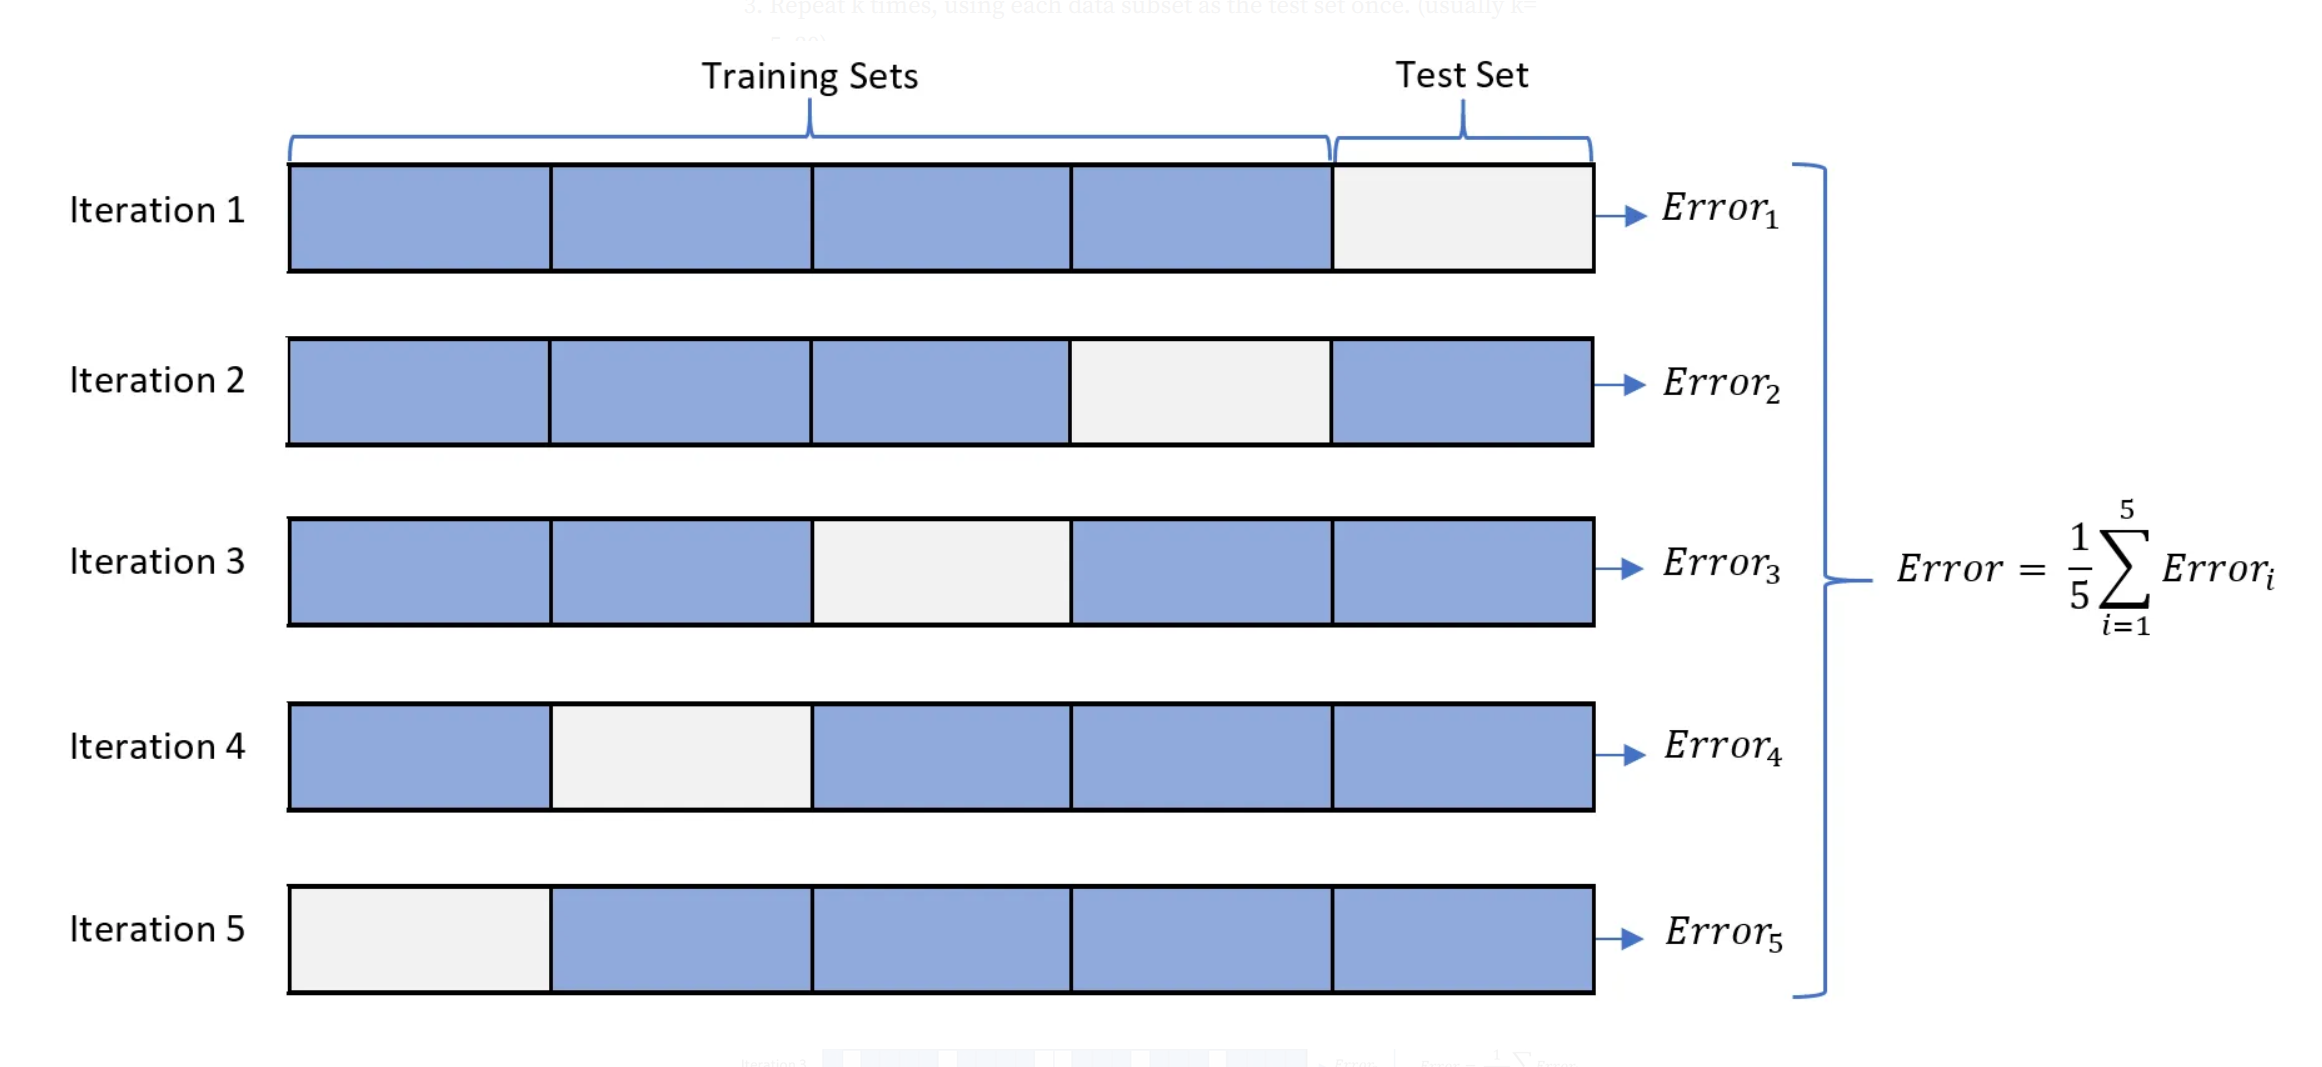
\includegraphics[scale=0.18]{5foldCV.png}
\centering
\caption{Example of k-fold Cross Validation with k=5 folds \cite{b4}}
\label{fig:kfoldCV}
\end{figure}

\newpage

In the cross validation process for both the decision tree and logistic regression models, the \lstinline{cv} parameter was set to \lstinline{None} meaning it uses the default of k=5 folds, and the \lstinline{scoring} parameter was set to \lstinline{accuracy} since that was the strategy chosen to determine the effectiveness of the models. The mean and standard deviation of the cross validation of both models was determined. 

To validate the \lstinline{cross_validate} function from sklearn, we also created our own cross validation function called \lstinline{perform_manual_cross_validation} that goes through the same algorithm of splitting the Iris data into folds, using one fold as the test data, and iterating through until all the folds have been used as test data. We ran this function on the same decision tree and linear regression models; the accuracy each iteration was printed and the mean and standard deviation of those accuracies were compared to when the \lstinline{cross_validate} function was used. 

Returning to using the \lstinline{cross_validate} function we changed the \lstinline{cv} parameter, setting it to the values of 3, 7, and 10 to see how the accuracy of the cross validated decision tree and linear regression models would change. We were especially interested in seeing how setting k=10 would affect accuracy because k=5 and k=10 are the more common fold values.


\section{Results}
\label{sec:results}

The mean and standard deviation accuracy values from performing 5-fold cross validation on our logistic regression and decision tree models are shown in Table~\ref{table:5FoldCV}

\begin{table}[h!]
\centering
\begin{tabular}{ c | c c }
Measure & Logistic Regression & Decision Tree \\
\hline
Mean & 0.973333 & 0.960000 \\
Standard Deviation & 0.036515 & 0.036515 \\
\end{tabular}
\caption{5-Fold Cross Validation Statistics for Logistic Regression and Decision Tree Models}
\label{table:5FoldCV}
\end{table}

It can be seen that the logistic regression model is slightly more accurate than the decision tree model, at 0.973 compared to 0.960. This lines up with our previous study; when the results of that linear regression model were briefly compared to that decision tree model, the logistic regression model was more accurate. Here, we used a more robust method of evaluating effectiveness of the models and found the same conclusion to be true.

The results of our own k-fold cross validation function \lstinline{perform_manual_cross_validation} produced similar results, seen in Table ~\ref{table:5FoldManualCV}. 

\begin{table}[h!]
\centering
\begin{tabular}{ c | c c }
Measure & Logistic Regression & Decision Tree \\
\hline
Mean & 0.953333 & 0.933333 \\
Standard Deviation & 0.038006 & 0.0.062361 \\
\end{tabular}
\caption{5-Fold Manual Cross Validation Statistics for Logistic Regression and Decision Tree Models}
\label{table:5FoldManualCV}
\end{table}

Although the values are not exactly the same as when the \lstinline{cross_validate} function was used, it still confirms that the logistic regression model is slightly more accurate than the decision tree model. The higher standard deviation values may be attributed to the way the data is being split into the folds; it is just splitting the Iris dataset into fifths without implementing a random order. 

The results of performing k-fold cross validation using sklearn and changing the number of folds are shown below. The additional k values of 3, 7, and 10 are used.

\begin{table}[h!]
\centering
\begin{tabular}{ c | c c }
Measure & Logistic Regression & Decision Tree \\
\hline
Mean (k=3) & 0.973333 & 0.96 \\
Standard Deviation (k=3)  & 0.023094 & 0.02 \\
Mean (k=5, default) & 0.973333 & 0.96 \\
Standard Deviation (k=5, default)  & 0.036515 & 0.036515 \\
Mean (k=7) & 0.959802 & 0.939703 \\
Standard Deviation (k=7)  & 0.074425 & 0.065443 \\
Mean (k=10) & 0.98 & 0.953333 \\
Standard Deviation (k=10)  & 0.044997 & 0.044997 \\
\end{tabular}
\caption{Cross Validation Statistics for Logistic Regression and Decision Tree Models (k=3, 5, 7, 10)}
\label{table:MultiFoldCV}
\end{table}

For all k-values, the logistic tree models consistently showed to have greater accuracy than the decision tree model. Between k=3 and k=5, the accuracy of both the models did not change. When k=7, the accuracy of both models decreased - this could be because the folds do not have the same amount of data, as 150 data points do not divide evenly between 7 groups, also causing more variance within the accuracy of the folds. When k=10, the accuracy of both models increases slightly compared to k=3 and k=5. This could be a sign of overfitting as each fold has much less data meaning that the training portion is increasingly bigger than the testing portion during each iteration. 



\section{Discussion}
\label{sec:discussion}
Through this investigation, we were able to confirm that the logistic regression model was more effective as a predictive model for the Iris dataset as compared with a decision tree model. Here, we used a more robust method of evaluating effectiveness of the models and found the same results. K-fold cross validation allows for a relatively quick confirmation of which model in question is more accurate as compared to other models. 

In the case of a larger dataset, using k=10 may be found to work better, The accuracy of both testing and training data could be observed to determine if overfitting is occurring. Also, this study used the entire Iris dataset as the portion used for the k-fold cross-validation. In the future, the Iris dataset could be split into test and train partitions, more similar to what was done in previous studies. Then, k-fold cross validation would only be performed on the training data and the results of that would finally be applied to the testing data.

\newpage

\begin{thebibliography}{00}
\bibitem{b1}
J. Brownlee, “A Gentle Introduction to k-fold Cross-Validation,” MachineLearningMastery.com. Accessed: Oct. 01, 2023. [Online]. Available: https://machinelearningmastery.com/k-fold-cross-validation/
\bibitem{b2}
L. Mueller and R. Hong, “Investigating Decision Trees,” Sep. 18, 2023.
\bibitem{b3}
L. Mueller and R. Hong, “Iris Classification Using Logistic Regression,” Sep. 25, 2023.
\bibitem{b4}
R. Patro, “Cross Validation: K Fold vs Monte Carlo,” Medium. Accessed: Oct. 05, 2023. [Online]. Available: https://towardsdatascience.com/cross-validation-k-fold-vs-monte-carlo-e54df2fc179b

\end{thebibliography}

\end{document}